\chapter{Methodology and Data Processing}
\label{chap:methodology}

This chapter describes the data processing pipeline and the technical methodology used by the Lectura platform. It covers input ingestion, text cleaning, prompt engineering, the asynchronous processing architecture, and the security and payment systems.

\section{Input Formats and Modalities}
To accommodate the varied workflows of university students, the Lectura platform was designed to accept several different types of input. Since students encounter course material in many formats, the ingestion engine is built as a separate module from the generation engine, allowing it to handle the following input types:

\begin{itemize}[label=\textendash]
    \item YouTube Video Transcripts: The primary source of educational content for many students. Lectura connects to YouTube's API to extract closed captions, capturing the spoken content of video lectures without requiring manual transcription.
    \item Document Uploads: Support for PDF, DOCX, and plain TXT files, covering everything from formatted research papers to basic textbook chapters.
    \item Raw Text Input: Users can also paste text directly into the interface, which is useful for short excerpts from forums, emails, or other fragmented sources.
    \item Future Audio Support: The architecture includes provisions for eventually supporting direct audio input via speech-to-text, which would enable processing of live classroom lectures.
\end{itemize}

\section{Transcript Cleaning and Sanitization}
Raw transcript data from YouTube is typically noisy. The XML output from the YouTube Data API contains HTML entities (e.g., \verb|&amp;|, \verb|&quot;|), embedded timestamps, non-speech markers ([Applause], [Music]), and fragmented sentences caused by automatic captioning.

If this uncleaned text is sent directly to a Large Language Model, the output quality drops significantly, often resulting in incoherent or hallucinated content. Therefore, the Lectura backend applies a multi-step cleaning process.

First, a regular expression engine removes HTML artifacts and filters out non-verbal markers. Second, the algorithm addresses sentence fragmentation by analyzing the time gaps between captions. When the gap between two consecutive timestamps exceeds 3.0 seconds, the system inserts a paragraph break. This grouping produces naturally flowing text from what was originally a fragmented subtitle file, and it preserves the semantic relationship between concepts that were discussed together.

One limitation of processing videos using only transcripts is that it relies entirely on what is spoken aloud. Educational videos often include important information on the screen, such as slide titles, math formulas, code snippets, or diagrams. To solve this, Lectura includes an optional feature to extract visual content. When a user selects the ``Read text on video screen'' option, the backend sends the video frames to the Google Gemini multimodal API along with the audio transcript. The model uses OCR to read the text that appears on the screen. This extracted text is then added to the prompt as extra context, prioritized if there is a conflict between the subtitles and the visual text.

\section{PDF Text Extraction}
PDF extraction presents a different engineering challenge compared to video transcripts. PDF files do not store text as a logical sequence of sentences; instead, they store coordinates that map individual characters onto a visual canvas. In a multi-column academic paper, a naive line-by-line parser would mix text from the left column with text from the right column, producing nonsensical output.

Lectura addresses this using spatial analysis (primarily through the \texttt{pdfplumber} library via Python microservices). The extraction process analyzes the x, y coordinates of character blocks on each page, calculates bounding boxes, and distinguishes between headers, body text, and footnotes. Page numbers, repeating footers, and marginal notes are identified and removed. For multi-column layouts, columns are sorted by their horizontal position, ensuring that the extracted text follows the natural top-to-bottom, left-to-right reading order.

\section{Prompt Engineering and Context Window Management}
Once the input has been cleaned and converted into a single text string, it enters the AI generation layer. Modern language models have fixed token limits, and attempting to send a very long transcript in a single API call can result in truncation or errors.

Lectura handles this through a sliding window chunking approach. If the input exceeds a defined maximum token threshold ($T_{\max}$), the text is divided into sequential chunks $C = \{c_1, c_2, \dots, c_k\}$, with each chunk overlapping the next by $O_{\text{lap}}$ tokens. The number of chunks $k$ for a text of length $L$ tokens is approximately:

\begin{equation}
    k = \left\lceil \frac{L - O_{\text{lap}}}{T_{\max} - O_{\text{lap}}} \right\rceil
\end{equation}

The precise chunking logic executed by the backend is documented in Algorithm~\ref{alg:sliding_window}.

\begin{algorithm}[htbp]
\caption{Sliding Window Context Overlap Extraction}
\label{alg:sliding_window}
\begin{algorithmic}[1]
    \REQUIRE Extracted text string $S$; Max token limit $T$; Overlap size $O$
    \ENSURE Array of text chunks $C$
    
    \STATE $\textit{tokens} \leftarrow \text{Tokenize}(S)$
    \STATE $L \leftarrow \text{Length}(\textit{tokens})$
    \STATE $C \leftarrow [ ]$
    \STATE $\textit{index} \leftarrow 0$
    
    \WHILE{$\textit{index} < L$}
        \STATE $\textit{end\_boundary} \leftarrow \min(\textit{index} + T, L)$
        \STATE $\textit{chunk} \leftarrow \textit{tokens}[\textit{index} \dots \textit{end\_boundary}]$
        \STATE $C\text{.append}(\textit{chunk})$
        
        \IF{$\textit{end\_boundary} == L$}
            \STATE \textbf{break}
        \ENDIF
        
        \STATE $\textit{index} \leftarrow \textit{index} + T - O$ \COMMENT{Shift backward by $O$ to retain context}
    \ENDWHILE
    
    \RETURN $C$
\end{algorithmic}
\end{algorithm}

Each chunk is then paired with a system prompt that defines the model's behavior. The system injects a fixed instruction header into every request (e.g., ``You are an academic tutor. Analyze the following content and format it strictly as Markdown Cornell notes.'').

Generating presentation slides introduces the strictest formatting requirements. The prompt enforces a specific JSON schema where each slide object includes a \texttt{slide\_type} field from a predefined list (e.g., \texttt{hero\_image}, \texttt{big\_stat}, \texttt{icon\_grid}). Content length constraints prevent slides from becoming text-heavy: for example, an \texttt{icon\_grid} slide must contain exactly three or four bullet points, each no longer than eight words.

The extraction pipeline from raw input to stored database entries is illustrated in Figure~\ref{fig:pipeline}.

\begin{figure}[htbp]
\centering
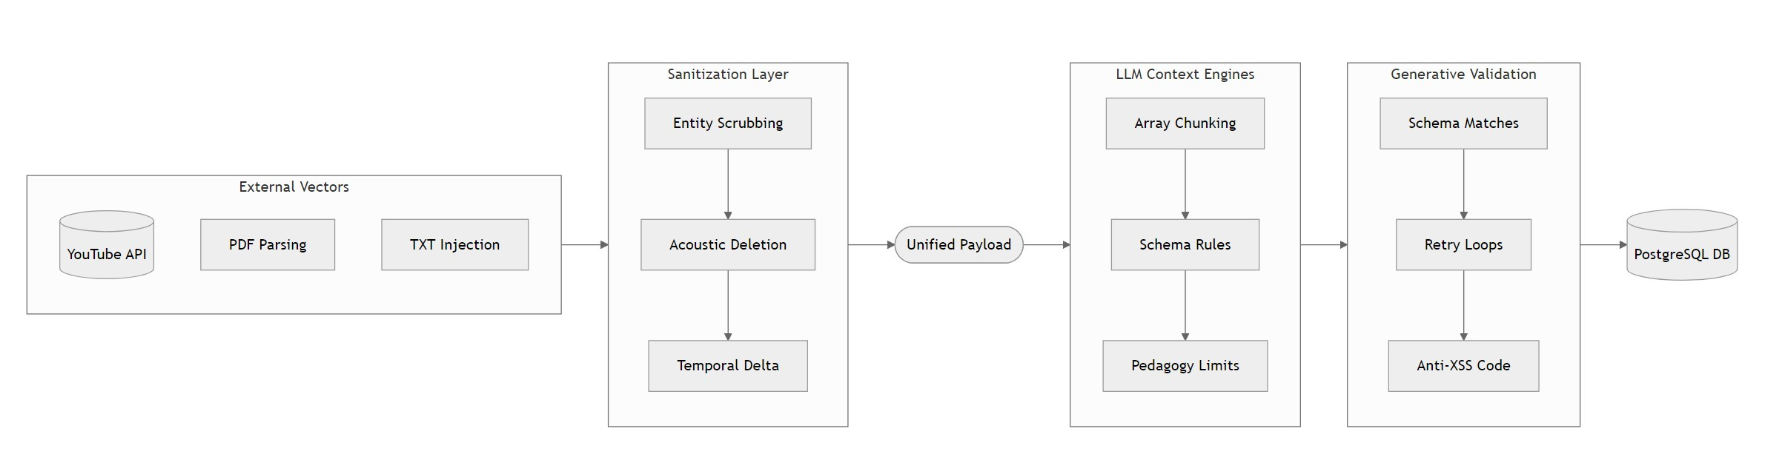
\includegraphics[width=\textwidth]{chapters/chapter03/images/figure3.png}
\caption{Overview of the data ingestion and processing pipeline.}
\label{fig:pipeline}
\end{figure}

\section{AI Prompt Engineering Strategy}
When working with large language models, prompt engineering becomes a core part of the system architecture. The Lectura backend takes the cleaned input data and runs it through a multi-stage prompting pipeline:

\begin{itemize}[label=\textendash]
    \item Hierarchical Summarization: When the input exceeds 15,000 tokens, the text is split into overlapping chunks, each summarized separately, and then combined via a second ``meta-prompt'' into a single coherent output.
    \item Bloom's Taxonomy Quiz Generation: The quiz prompts instruct the model to generate higher-order questions that require analysis, application, and synthesis rather than simple recall.
    \item Flashcard Generation: Flashcard prompts force the model to break down complex topics into short, focused question-answer pairs, each targeting a single concept.
    \item Chain-of-Thought (CoT) Prompting: For dense technical content, the backend includes instructions that make the model show its reasoning steps before producing the final output, reducing the chance of hallucinated content.
\end{itemize}

\section{System Design Approach}
Lectura was designed following modern cloud-native architectural principles. The architecture separates the application into two main layers: a client-side React frontend and a concurrent Go-based backend. A ``web-first'' approach was chosen, aligning with the typical usage patterns of university students who primarily use laptops for content consumption. To maintain usability on smaller screens, the interface uses Tailwind CSS with breakpoint-driven responsive layouts.

\section{Worker Pool Architecture and Asynchronous Processing}
Processing a two-hour lecture — generating summaries, a quiz, and a flashcard deck — typically takes between 10 and 60 seconds due to LLM response times. If this processing were handled synchronously within a standard HTTP request, users would experience connection timeouts and unresponsive browser tabs.

To avoid this, Lectura uses a Worker Pool pattern. When a user submits content for processing, the backend creates a ``Job Ticket'' in the database queue and immediately returns a \texttt{202 Accepted} response to the frontend. In the background, a pool of Go goroutines monitors the queue. When a worker picks up a job, it handles the Gemini API calls, parses the responses, and stores the finished artifacts in the database. The workers also implement Exponential Backoff retries to handle API rate limits from external providers.

The choice of Go was motivated by its M:N goroutine scheduler. In conventional applications, each concurrent task requires an OS thread with a stack allocation of roughly 1--2 MB. Go goroutines start with approximately 2 KB. When a goroutine blocks on an HTTP request to the Gemini API, the scheduler moves it off the OS thread in $O(1)$ time, without requiring a kernel-level context switch. The memory required scales as follows:

\begin{equation}
    \text{Mem}_{\text{traditional}} = N \times (2 \cdot 10^6 \text{ Bytes}) \gg \text{Mem}_{\text{Go}} = N \times (2 \cdot 10^3 \text{ Bytes})
\end{equation}

This roughly 1000x reduction in per-connection memory cost allows Lectura to handle traffic spikes during exam periods without expensive infrastructure.

\section{WebSocket Real-Time Updates}
Since the content generation happens in background workers, the React frontend needs a way to receive progress updates in real time. Instead of polling the server repeatedly, Lectura uses WebSockets for bidirectional communication.

When a user submits a generation request, the React client opens a persistent WebSocket connection. As the background worker progresses through the job, it pushes status updates through this channel — events like \texttt{JOB\_QUEUED}, \texttt{TRANSCRIPT\_SANITIZED}, and \texttt{GENERATION\_COMPLETE}. Using WebSockets avoids the overhead of repeated HTTP polling, where each request includes 700--1200 bytes of headers. With the RFC 6455 WebSocket protocol, subsequent data frames carry only a 2-to-10 byte framing header, reducing bandwidth used for status updates by roughly 98\%.

\section{Database Schema and Output Validation}
The PostgreSQL schema balances relational integrity with the flexibility needed for AI-generated content. User accounts and authentication data are normalized to Third Normal Form (3NF). The artifacts produced by the LLM are stored using PostgreSQL's native JSONB column type, which allows prompt format updates without database migrations while supporting efficient queries through JSONB indexing.

AI-generated output is not always perfectly formatted. The model may occasionally drop required delimiters. Lectura includes a validation step before storing any generated content. If a response fails validation, the worker retries the request. All content is sanitized to remove potential XSS payloads before being written to the database.

\section{Interactive State Management and Inline Editing}
The presentation feature treats generated slides not as static outputs but as editable documents. The frontend uses a \texttt{SlideViewer} component that maintains the slide data as a nested JSON state. An \texttt{EditableText} component allows inline editing: when a user clicks on a slide heading, the static element is replaced with an auto-resizing text area.

To avoid sending a separate HTTP request for every keystroke, the application uses a debounce mechanism. The debounce hook waits for a set interval (e.g., 1000ms) after the last keystroke before sending the updated content to the backend. The flow is illustrated in Figure~\ref{fig:debounce_flow}.

\begin{figure}[htbp]
\centering
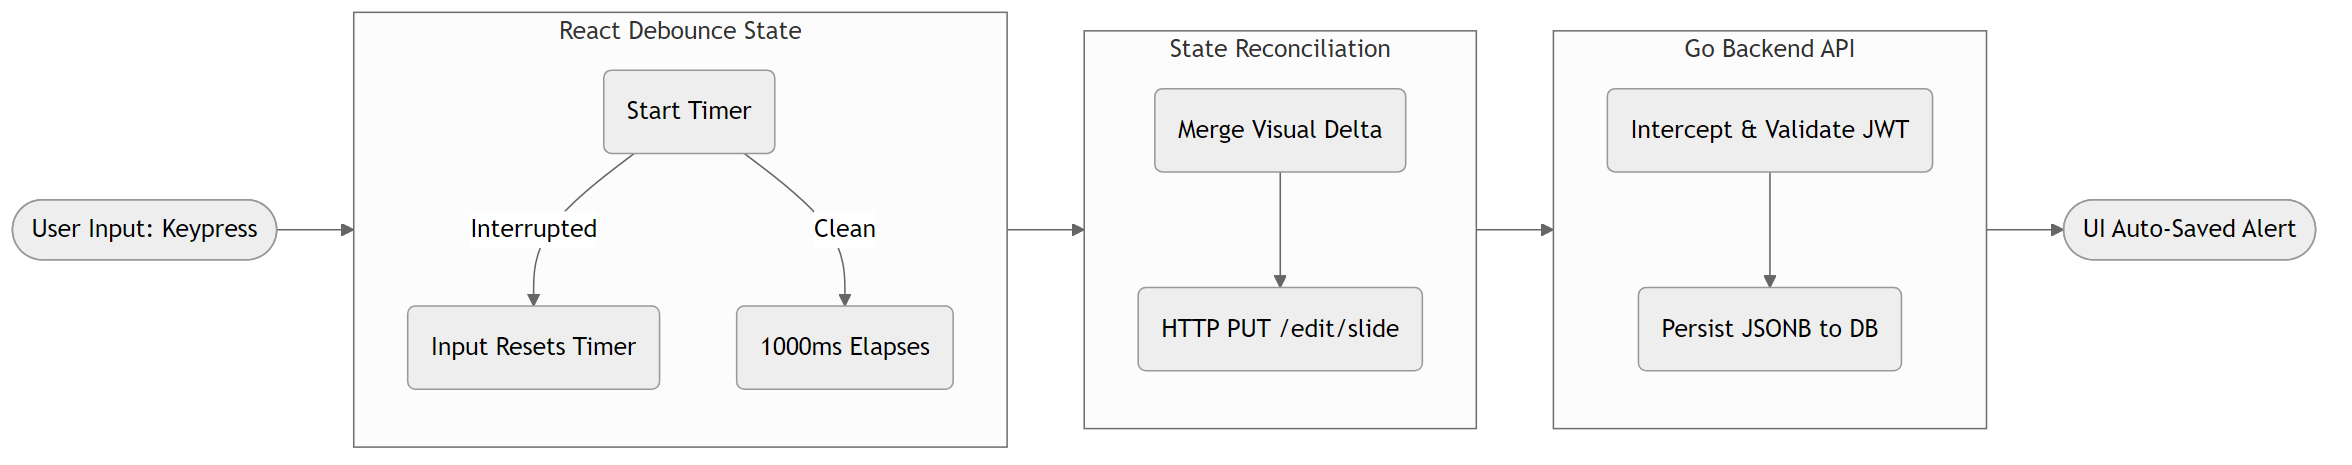
\includegraphics[width=\textwidth]{chapters/chapter04/images1/debounce.png}
\caption{State flow diagram for the Presentation Inline Editor debounce mechanism.}
\label{fig:debounce_flow}
\end{figure}

\section{Security and Payment Integration}
Lectura uses JWT authentication with short-lived access tokens (15-minute expiry) and longer-lived refresh tokens. CORS policies restrict which domains can interact with the API. All database queries use parameterized statements to prevent SQL injection, and both AI-generated and user-submitted content is sanitized to prevent XSS attacks. Rate limiting on authentication endpoints protects against brute-force login attempts.

To support the ongoing costs of running LLMs, Lectura includes a tiered subscription system using Stripe. Users start on a free tier with limited generations per month, and premium plans increase these limits. The payment processing is handled server-side using the Stripe Go SDK, and Stripe webhooks update the user's subscription status after successful payment. Because the payment forms are hosted by Stripe, cardholder data never touches the Lectura servers, simplifying PCI DSS compliance.